

\chapter{RESULT AND DISCUSSION}

\hspace{0.9cm} The implementation described in the previous section leads to a lot of results and requires explanation.

\begin{itemize}
	\item The project is mainly to improve execution speed of analysis of datasets. It deals with converting the datasets from its numerical form to the 8 bit grayscale colour domain\\
	\begin{enumerate}
		\item Graphs
		\item Result
	\end{enumerate}
%	1. Graphs\\ 
%	
%	2. Result: 
%	3.
%	
%	a. Conclusion, b. Application; 
	
	\item deals with the analysis and simulation studies.
	\item Advantages and disadvantages.
	\begin{figure}[h!]
		\centering	
		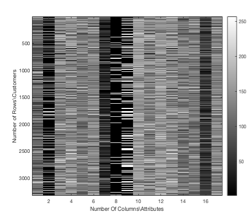
\includegraphics[width=2.5in]{1.png} % e.g. insert ./image for image.png in the working directory, adjust scale as necessary
		\caption{Customer records and attributes as an image.}
		\label{fig:1} % insert suitable label, this is used to refer to a fig from within the text as shown above
		
	\end{figure}\\
	\begin{figure}[h!]
		\centering	
		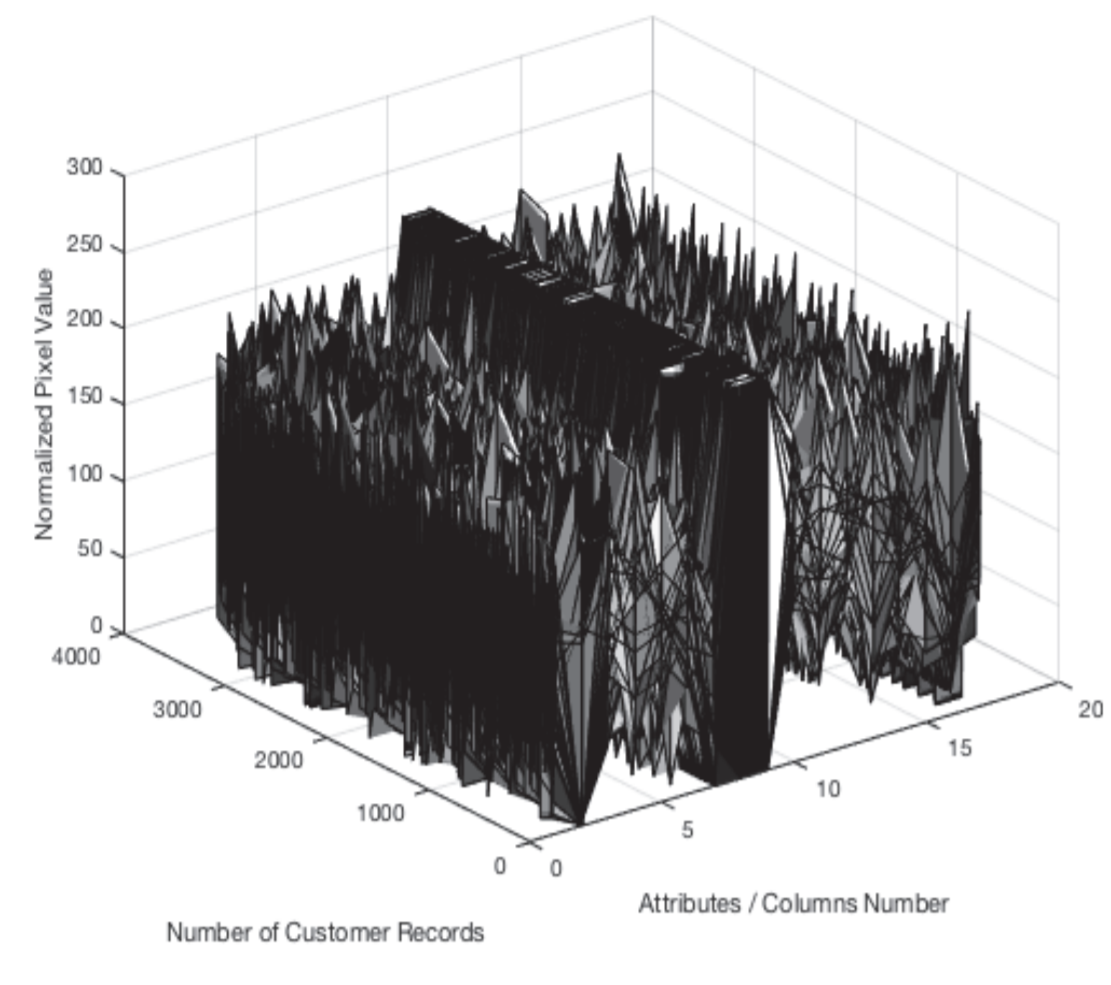
\includegraphics[width=2.5in]{2.png} % e.g. insert ./image for image.png in the working directory, adjust scale as necessary
		\caption{ 3D surface plot of customer records and attributes.}
		\label{fig:2} % insert suitable label, this is used to refer to a fig from within the text as shown above
		
	\end{figure}
	\begin{figure}[h!]
		\centering	
		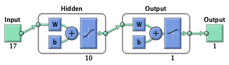
\includegraphics[width=2.0in]{3.png} % e.g. insert ./image for image.png in the working directory, adjust scale as necessary
		\caption{ Structure of neural network.}
		\label{fig:3} % insert suitable label, this is used to refer to a fig from within the text as shown above
		
	\end{figure}
	
	The neural network is implemented with the Neural
	Network Toolkit (NNT) \cite{citation-11} in MATLAB \cite{citation-10}. The NNT
	contains predefined types of neural networks for clustering,
	fitting, pattern recognition, and time series. These types make
	it possible to instantly deploy the neural networks, which
	otherwise would take considerable time to set up. The NNT
	handles all initializing of weights and other trivial processes.
	We use the pattern recognition pre-set for the neural network
	so that we can detect trends and patterns via neural networks.
	As we mentioned earlier, we are using the supervised
	learning approach since we have a labelled dataset for churn
	analysis. For creating the neural network, we have to select
	certain parameters such as \textless{} parameter x, parameter y \textgreater{}. We
	have to select the number of hidden layers. This can have an
	impact on the accuracy of prediction that is obtained. We use
	10 hidden layers, which is the default number of layers.
	The selected pre-set pattern recognition neural network in
	the neural network is implemented with the Neural Network
	Toolkit (NNT) \cite{citation-11} in MATLAB \cite{citation-10}. The NNT contains
	predefined types of neural networks for clustering, fitting,
	pattern recognition, and time series. These templates make it
	possible to instantly deploy neural networks, which otherwise
	would take considerable time to set up. The \cite{citation-11} handles all
	initialization of weights and other trivial processes. are handled
	by the NNT\cite{citation-11}.
	NNT\cite{citation-11} has to be trained like any other network for creating
	a model. We use Scaled conjugate gradient back propagation
	for supervised training \cite{citation-6}. This is the default algorithm for
	the pattern recognition neural network in the NNT. The neural
	network as illustrated in Fig. 3 has 17 inputs, since the input
	customer attributes are 17. It gives a binary output as evident
	in \ref{fig:3}.
	We observed varying accuracies since the weights are
	all initialized randomly. Anybody wishing to recreate the
	experiment may not get exact matching results due to this
	randomness. But, the accuracy of prediction should be nearby
	in the neighbourhood of 1–2\% or more
	\cite{citation-8}.
	
	\begin{table}[]
		\centering
		\caption{EXECUTION TIME ON EXPERIMENTAL SYSTEMS}
		\label{table-2}
		\vspace{0.9cm}
		\begin{tabular}{|l|l|l|}
			\hline
			Computer description   & \begin{tabular}[c]{@{}l@{}}CPU execution\\ time (seconds)\end{tabular} & \begin{tabular}[c]{@{}l@{}}GPU execution\\ time (seconds)\end{tabular} \\ \hline
			High End Custom PC     & 0.001553                                                               & 0.001051                                                               \\ \hline
			MacBook Air Early 2015 & 0.004755                                                               & N/A                                                                    \\ \hline
		\end{tabular}
	\end{table}
\end{itemize}

